\documentclass[]{article}

\usepackage[utf8]{inputenc}
\usepackage{amsmath}
\usepackage{amssymb}
\usepackage{amsthm}
\usepackage{amsfonts}
\usepackage{graphicx}
\usepackage{capt-of}
\usepackage{listings}
\usepackage{siunitx}
\usepackage[section]{placeins}
\usepackage[T1]{fontenc}
\usepackage{lmodern}
\usepackage{color}
\usepackage{hyperref}
\usepackage{epstopdf}
\usepackage{matlab}
\usepackage{float}


% Oppgavenummerering %
\renewcommand\thesection{Task \arabic{section}}
\renewcommand\thesubsection{\alph{subsection})}

% Bevis
\newcommand\TombStone{\rule{.5em}{.5em}}
\renewcommand\qedsymbol{\TombStone}

\title{\huge{TTK4250 – Sensor Fusion} \\ \LARGE{Assignment 1}}
\author{Sigurd Totland | MTTK}

\begin{document}
\maketitle

\section{}
Let the cdf of $Y$ be $P_Y(y)$. From its definition we obtain
\begin{align*}
P_Y(y) =\Pr(Y \leq y)=\Pr(P(X) \leq y).
\end{align*}
We assume monotonicity of $P(X)$ which means that its inverse is defined. By this we obtain
\begin{align*}
P_Y(y) &= \Pr(P^-(P(X)) \leq P^-(y)) \\
&= \Pr(X \leq P^-(y)) \\
&= P(P^-y)) \\
&= y.
\end{align*}
Since the cdf of $Y$ is a unit ramp, $Y$ is uniformly distributed. \qed

\section{}
\subsection{}
The probability generating function for a discrete random variable is defined as
\begin{align}
G(t) = \sum_{x=0}^{\infty}f_X(x)t^x.
\end{align}
Using the power series definition $e^t = \sum_{x=0}^{\infty}\frac{t^x}{x!}$ and the probability mass function of the Poisson distribution $f_X(x) = \frac{\lambda^x e^{-\lambda}}{x!}$ we obtain
\begin{align*}
G(t) &= \sum_{x=0}^{\infty}\frac{\lambda^x e^{-\lambda}}{x!}t^x \\
&= e^{-\lambda}\sum_{x=0}^{\infty}\frac{(\lambda t)^x}{x!} \\
&= e^{-\lambda}e^{\lambda t} \\
&= e^{\lambda(t - 1)}. \qed
\end{align*}

\subsection{}
The pmf of the Binomial distribution is $f_X(x)= \binom{n}{x}r^x(1-r)^{n-x}t^x$. We then obtain the pgf
\begin{align*}
G(t) &= \sum_{x=0}^{n}f_X(x)t^x \\
&= \sum_{x=0}^{n}\binom{n}{x}r^x(1-r)^{n-x}t^x \\
&= \sum_{x=0}^{n}\frac{n!}{x!(n-x)!}(rt)^x(1-r)^{n-x} \\
&= [(1-r) + rt]^n,
\end{align*}
where the last result is obtained using the binomial theorem. \qed

\subsection{}
Letting $r = \frac{\lambda}{n}$ and taking the limit as $n\rightarrow\infty$ we obtain
\begin{align*}
\lim_{n\rightarrow \infty}[(1-\frac{\lambda}{n}) + \frac{\lambda}{n}t]^n = (1 + \frac{\lambda(t-1)}{n})^n = e^{\lambda(t-1)}
\end{align*}
which happens to be the pgf for the Poisson distribution. Informally speaking, this is because a Poisson distribution is just an infinite sequence of Bernoulli trials, so $n$ becomes infinite instead of finite.

\subsection{}
\textbf{Using PGF}\\
For the sum of (in this case two) independent random variables, the pgf becomes
\begin{align}
G_N(t) = G_{N_1}(t)G_{N_2}(t),
\end{align}
i.e. the product of the respective pgfs. For Poisson distributed variables $N_1$ and $N_2$ this becomes
\begin{align}
G_N(t)=e^{\lambda_1(t-1)}e^{\lambda_2(t-1)} =e^{(\lambda_1 + \lambda_2)(t-1)}.
\end{align}
N is thus Poisson distributed with probability parameter $\lambda$. \qed\\
\textbf{Using PMF}\\
For the pmf we instead have
\begin{align*}
f_N(t) &= (f_{N_1} * f_{N_2})(t) \\
&= \sum_{x=0}^{t}\frac{\lambda_1^xe^{-\lambda_1}}{x!}\frac{\lambda_2^{t-x}e^{-\lambda_2}}{(t-x)!} \\
&= \frac{e^{-(\lambda_1 + \lambda_2)}}{t!} \sum_{x=0}^{t}\frac{t!}{x!(t-x)!}\lambda_1^x\lambda_2^{t-x} \\
&= \frac{(\lambda_1 + \lambda_2)^t e^{-(\lambda_1+\lambda_2)}}{t!} \\
&= \text{Poisson}(t; \lambda_1 + \lambda_2). \qed
\end{align*}
Clearly, using the probability generating function is much simpler than just the probability mass function. This is due to the fact that random variables addition becomes simple multiplication in the pgf case, but becomes a convolution operation in the pmf case which is generally much harder to compute.
\section{}
\subsection{}
We first rewrite the expression as
\begin{equation}\begin{aligned}
p(t_1|t_1 \geq t_0) = \Pr(T>t_1|T>t_0).
\end{aligned}\end{equation}
From Bayes' theorem we obtain
\begin{equation}\begin{aligned}
\Pr(T>t_1|T>t_0) = \frac{\Pr(T>t_0|T>t_1)\Pr(T>t_1)}{\Pr(T>t_0)}.
\end{aligned}\end{equation}
Assuming $t_1 > t_0$, if $T>t_1$, then $T>t_0$, so $\Pr(T>t_0|T>t_1) = 1$. We then get
\begin{equation}\begin{aligned}
\Pr(T> t_1|T>t_0) = \frac{\Pr(T>t_1)}{\Pr(T>t_0)}.
\end{aligned}\end{equation}
Using the pdf of the exponential distribution, we finally obtain
\begin{equation}\begin{aligned}
\Pr(T> t_1|T>t_0) = \frac{e^{-\lambda t_1}}{e^{-\lambda t_0}} = e^{-\lambda(t_1-t_0)}. \qed
\end{aligned}\end{equation}
This result is known as memorylessness. To interpret what this means intuitively, we must first how the exponential distribution is interpreted. In this problem, the probability density function $p(t)$ tells us the probability that \textit{the next boat} will arrive in $t$ minutes. Memorylessness in this regard then means that even though we might have waited some time $t_0$ for a boat to arrive, the probability that it will come in $t_1 - t_0$ minutes does not change. It is useful for us, because this is how the world works when the boats are independent. (Had they not been, if they for instance worked together to keep their frequence of arrival as constant as possible, we would not have the memorylessness property.)

\subsection{}
We use the result from example 2.9, i.e. that a sum of $n$ exponentially distributed variables are gamma distributed with scale parameter $\frac{1}{\lambda}$ and shape parameter $n$. Likewise, we obtain
\begin{equation}\begin{aligned}
t_n - t_0 = \sum_{i=1}^{n}t_i-t_{1-i} \sim \text{Gamma}(n, \frac{1}{\lambda}).
\end{aligned}\end{equation}

\subsection{}
Due to the memorylessness property, this is the same as asking what the probability is that boat $n+1$ arrives after $T - t_n$ time from now, i.e.
\begin{equation}\begin{aligned}
\Pr(t_{n+1} > T - t_n) = 1-\Pr(t_{n+1} \leq T - t_n)
\end{aligned}\end{equation}
Since the CDF of the exponential function is $1 - e^{-\lambda t}$, we get that this probability equals
\begin{equation}\begin{aligned}
1-\Pr(t_{n+1} \leq T - t_n) = 1 - 1 + e^{-\lambda(T - t_n)} = e^{-\lambda(T-t_n)}.
\end{aligned}\end{equation}

\section{}
\subsection{}
The moment generating function of $z$ is
\begin{equation}\begin{aligned}
M_z(t)
= \text{E}[e^{t^\top \Sigma^{-\frac{1}{2}}}(x-\mu)]
= e^{-t ^\top \Sigma^{-\frac{1}{2}}\mu}\text{E}[e^{t^\top \Sigma^{-\frac{1}{2}}x}].
\end{aligned}\end{equation}
We notice that $\text{E}[e^{t^\top \Sigma^{-\frac{1}{2}}x}]$ is the moment generating function of the random variable $\Sigma^{-\frac{1}{2}x}$. By linearity of the multivariate Gaussian, we know that
\begin{equation}\begin{aligned}
\Sigma^{-\frac{1}{2}}x \sim \mathcal{N}(
\Sigma^{-\frac{1}{2}}\mu,
\Sigma^{-\frac{1}{2}}\Sigma(\Sigma^{-\frac{1}{2}})^\top).
\end{aligned}\end{equation}
Furthermore, using the property $\Sigma^{\frac{1}{2}}(\Sigma^{\frac{1}{2}})^{\top} = \Sigma$ we have
\begin{equation}\begin{aligned}
\Sigma^{-\frac{1}{2}}\Sigma(\Sigma^{-\frac{1}{2}})
= \Sigma^{-\frac{1}{2}}\Sigma^{\frac{1}{2}}\Sigma^{\frac{1}{2}}(\Sigma^{-\frac{1}{2}})
= \text{I}.
\end{aligned}\end{equation}
We also know that the moment generating function of any multivariate gaussian with expectation $\mu_0$ and variance $\Sigma_0$ is $M(t) = e^{t^\top(\mu_0 + \frac{1}{2}\Sigma_0 t)}$. Hence,
\begin{equation}\begin{aligned}
M_z(t) =
e^{-t^\top \Sigma^{-\frac{1}{2}}\mu}
e^{t^\top \Sigma^{-\frac{1}{2}}\mu}
e^{\frac{1}{2}t^\top\text{I}t}.
\end{aligned}\end{equation}
From this, we deduce that $z \sim \mathcal{N}(0, \text{I})$, i.e. $z$ is standard normal distributed.

\subsection{}
Since $z_i \sim \mathcal{N}(0, 1)$, this problem closely follows example 2.11. Since the square function is not invertible, we need to define both
\begin{equation}\begin{aligned}
\mathbf{f}^{-1}_1 = \sqrt{y_i} \quad \text{and} \quad \mathbf{f}^{-1}_2 = -\sqrt{y_i}.
\end{aligned}\end{equation}
Their jacobians are
\begin{equation}\begin{aligned}
\mathbf{F}^{-1}_1 = \frac{1}{2\sqrt{y_i}} \quad \text{and} \quad \mathbf{F}^{-1}_2 = -\frac{1}{2\sqrt{y_i}}.
\end{aligned}\end{equation}
By applying theorem 2.4.1, we arrive at the pdf
\begin{equation}\begin{aligned}
h(y_i)
= \frac{1}{\sqrt{2\pi}}\left[\frac{1}{2\sqrt{y_i}}e^{-\frac{1}{2}\sqrt{y_i}^2}e^{-\frac{1}{2}(-\sqrt{y_i}^2)}\right]
= \frac{1}{\sqrt{2 \pi y_i}}e^{-\frac{y_i}{2}},
\end{aligned}\end{equation}
just like in the example. This is the pdf of a $\chi^2$ distribution with $1$ degree of freedom.

\subsection{}
From the previous task, we know that $y_i$ is $\chi^2$ with $k=1$ degree of freedom. The MGF of any $\chi^2$ variable is $(1-2t)^{-\frac{1}{2}}$, so in this case $M_{y_i}(t) = (1-2t)^{-\frac{1}{2}}$. The MGF of $y=\sum_{i}y_i$ is then
\begin{equation}\begin{aligned}
M_y(t)
&= \text{E}[ e^{t \sum_{i}y_i}] \\
&= \prod_i \text{E}[ e^{t y_i}] \\
&= \prod_i (1 - 2t)^{-\frac{1}{2}} \\
&= (1 - 2t)^{-\frac{n}{2}}
\end{aligned}\end{equation}
where $n$ is the number of random variables in $y$. In other words, $y$, the \textit{Mahalanobis distance} from $x$ to $\mu$, is $\chi^2$ distributed with $n$ degrees of freedom.

\section{}
\subsection{}
We know that $p(z^c)$ is the pdf of $z^c$ and $p(z^c|x)$ is simply the pdf of $z^c$ \textit{given} the state $x$. From equation (4.71) in the book, we know this distribution is $\mathcal{N}(z^c; H \bar x, R)$, i.e. $p(z^c|x) = \mathcal{N}(z^c; H \bar x, R)$.

\subsection{}
This result follows from the proof of theorem 3.3.1 in the book. Like in the proof, we have that $p(z^c|x) = \mathcal{N}(z^c; Hx, R)$, and in addition, $x \sim \mathcal{N}(x; \bar x, P)$. As such, $p(x, z^c) = p(z^c|x)p(x) = \mathcal{N}(z^c; Hx, R) \mathcal{N}(x; \bar x, P)$. The proof then goes on in equation (3.13) to rewrite the quadratic form of this distribution to
\begin{equation}\begin{aligned}
(x - \hat x)^\top P^{-1}(x-\bar x) + (z^c - H^c x)^{\top} (R^c)^{-1}(z^c - H^c x) \\
=
\begin{bmatrix}
x - \bar x \\
z^c - H^c \bar x
\end{bmatrix}^\top
\begin{bmatrix}
P & P(H^c)^\top \\
H^c P & H^cP(H^c)^\top + R^c
\end{bmatrix}^{-1}
\begin{bmatrix}
x - \bar x \\
z^c - H^c \bar x
\end{bmatrix}
\end{aligned}\end{equation}
which we (and the proof) recognize as the quadratic form of a Gaussian. In other words, $p(z^c,x)$ is indeed Gaussian. \qed

\subsection{}
We know that $\text{E}[z^c] = \text{E}[Hx + v] = H\text{E}[x] + \text{E}[v] = H \bar x$.
From theorem 3.2.3, with
\begin{equation}\begin{aligned}
\begin{bmatrix}
P_{xx} & P_{xy} \\
P_{xy}^\top & P_{yy}
\end{bmatrix}
=
\begin{bmatrix}
P & P(H^c)^\top \\
H^c P & H^cP(H^c)^\top + R^c
\end{bmatrix}
\end{aligned}\end{equation}
we then have that
\begin{equation}\begin{aligned}
p(z^c) = \mathcal{N}(z^c;\mu_{z^c}, P_{yy}) = \mathcal{N}(z^c;H \bar x, H^cP(H^c)^\top + R^c).
\end{aligned}\end{equation}
Furthermore, the theorem tells us that
\begin{equation}\begin{aligned}
\mu_{x|z^c} &= \bar x + P_{xx}P_{yy}^{-1}(z^c - \mu_{z^c}) \\
&= \bar x + P(H^cP(H^c)^\top + R^c)^{-1}(z^c - \bar x)
\end{aligned}\end{equation}
and
\begin{equation}\begin{aligned}
P_{x|z^c} &= P_{xx} - P_{xy}P_{yy}^{-1}P_{xy}^\top \\
&= P - H^cP(H^cP(H^c)^\top + R^c)^{-1}P(H^c)^\top
\end{aligned}\end{equation}
and then the conditional
\begin{equation}\begin{aligned}
p(x|z^c) &= \mathcal{N}(x; \mu_{x|z^c}, P_{x|z^c}) \\
&= \mathcal{N}(x; \bar x + P(H^cP(H^c)^\top + R^c)^{-1}(z^c - \mu_{z^c}), \\
& P - H^cP(H^cP(H^c)^\top + R^c)^{-1}P(H^c)^\top). \\
\end{aligned}\end{equation}

\subsection{}
$F$ is not specified to be non-singular, which is required to be able to apply theorem 3.2.3. (In the proof, we need to take the inverse of $F$). If it \textit{is} non-singular, it should probably be possible to derive the same result, just replacing $H$ with $F$ and $R^c$ with $Q$ to obtain
\begin{equation}\begin{aligned}
p(x^+) = \mathcal{N}(x^+;F \bar x, F^cP(F^c)^\top + Q^c).
\end{aligned}\end{equation}
For $p(x|z^r)$ we get the corresponding result,
\begin{equation}\begin{aligned}
p(x|z^r) &= \mathcal{N}(x; \mu_{x|z^r}, P_{x|z^r}) \\
&= \mathcal{N}(x; \bar x + P(H^rP(H^r)^\top + R^r)^{-1}(z^r - \mu_{z^r}), \\
& P - H^rP(H^rP(H^r)^\top + R^r)^{-1}P(H^r)^\top). \\
\end{aligned}\end{equation}

\subsection{}
From theorem 2.6.1, we know that the MMSE estimator is pretty much just the expected value, i.e.
\begin{equation}\begin{aligned}
\hat x_{\text{MMSE}} = \mu_{x|z^c} =\bar x + P_{xx}P_{yy}^{-1}(z^c - \mu_{z^c}).
\end{aligned}\end{equation}
The MAP estimator on the other hand is given by
\begin{equation}\begin{aligned}
\hat x_{\text{MAP}} = \arg \max_x p(x|z^c).
\end{aligned}\end{equation}
According to the book, the MAP estimator has a closed form solution when estimating the expected value of a Gaussian. For more general systems however, we must resort to search techniques like Newton's method or steepest descent.

\subsection{ and \quad g)}
% This LaTeX was auto-generated from MATLAB code.
% To make changes, update the MATLAB code and export to LaTeX again.

\sloppy
\epstopdfsetup{outdir=./}
\graphicspath{ {./5ef/assignment1task5ef_images/} }

\begin{matlabcode}
% initialize the values
x_bar = zeros(2,1)
\end{matlabcode}
\begin{matlaboutput}
x_bar =
     0
     0

\end{matlaboutput}
\begin{matlabcode}
P = 25 * eye(2)
\end{matlabcode}
\begin{matlaboutput}
P =
    25     0
     0    25

\end{matlaboutput}
\begin{matlabcode}

H_r = eye(2)
\end{matlabcode}
\begin{matlaboutput}
H_r =
     1     0
     0     1

\end{matlaboutput}
\begin{matlabcode}
H_c = eye(2)
\end{matlabcode}
\begin{matlaboutput}
H_c =
     1     0
     0     1

\end{matlaboutput}
\begin{matlabcode}

R_c = [79, 36; 36, 36]
\end{matlabcode}
\begin{matlaboutput}
R_c =
    79    36
    36    36

\end{matlaboutput}
\begin{matlabcode}
R_r = [28, 4; 4, 22]
\end{matlabcode}
\begin{matlaboutput}
R_r =
    28     4
     4    22

\end{matlaboutput}
\begin{matlabcode}

z_c = [2; 14]
\end{matlabcode}
\begin{matlaboutput}
z_c =
     2
    14

\end{matlaboutput}
\begin{matlabcode}
z_r = [-4; 6]
\end{matlabcode}
\begin{matlaboutput}
z_r =
    -4
     6

\end{matlaboutput}
\begin{matlabcode}

% set up for plotting ellipses
Npts = 100; % number of points around the circle
circle = [cos( 0:(2*pi/Npts):(2*pi) ); sin( 0:(2*pi/Npts):(2*pi) )];

% initial 1 sigma ellipses
figure(1); clf; hold on; grid on;
data = x_bar + chol(P)' * circle;
plot(data(1,:), data(2, :), 'DisplayName','prior')

% measurements
scatter(z_c(1), z_c(2), 'DisplayName', 'z_c')
scatter(z_r(1), z_r(2), 'DisplayName', 'z_r')

legend()
\end{matlabcode}
\begin{center}
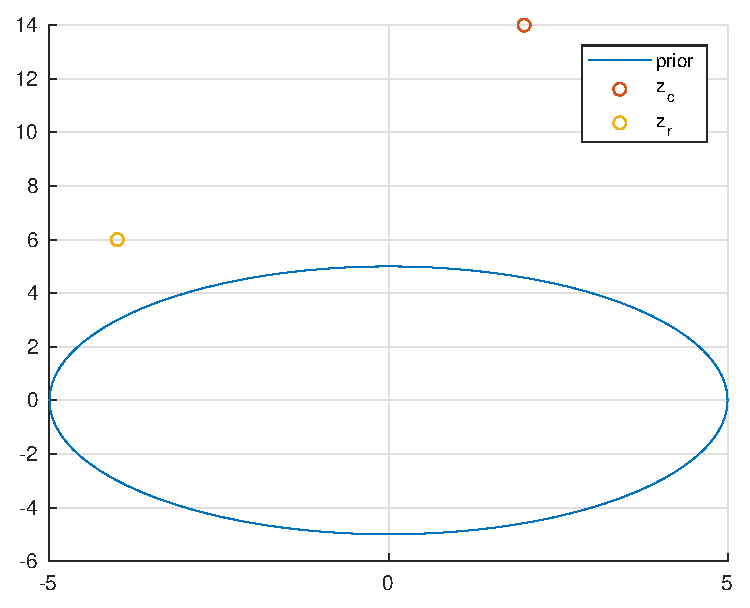
\includegraphics[width=\maxwidth{56.196688409433015em}]{figure_0}
\end{center}


\begin{matlabcode}
% You can make some functions to ease the conditionioning
% FILL IN THE DOTS ...
condition_mean = @(x_bar, z, P, H, R) x_bar + P*(H*P*H' + R)^(-1)*(z-x_bar);
condition_cov = @(P, H, R) P - H*P*(H*P*H' + R)^(-1)*P*H';
\end{matlabcode}


\begin{matlabcode}
% task 5 (f)
% FILL IN FOR THE DOTS ...

% condition on camera
x_bar_c = condition_mean(x_bar, z_c, P, H_c, R_c)
\end{matlabcode}
\begin{matlaboutput}
x_bar_c =
   -1.8918
    6.8542

\end{matlaboutput}
\begin{matlabcode}
P_c = condition_cov(P, H_c, R_c)
\end{matlabcode}
\begin{matlaboutput}
P_c =
   17.4475    4.4572
    4.4572   12.1236

\end{matlaboutput}
\begin{matlabcode}

% condition on radar
x_bar_r = condition_mean(x_bar, z_r, P, H_r, R_r)
\end{matlabcode}
\begin{matlaboutput}
x_bar_r =
   -2.1414
    3.3737

\end{matlaboutput}
\begin{matlabcode}
P_r = condition_cov(P, H_r, R_r)
\end{matlabcode}
\begin{matlaboutput}
P_r =
   13.1313    1.0101
    1.0101   11.6162

\end{matlaboutput}
\begin{matlabcode}

% Plot 1 sigma ellipses
figure(2); clf; hold on; grid on;

data = x_bar + chol(P)' * circle;
plot(data(1,:), data(2, :), 'DisplayName','prior')

data = x_bar_c + chol(P_c)' * circle;
plot(data(1,:), data(2, :), 'DisplayName', 'c')

data = x_bar_r + chol(P_r)' * circle;
plot(data(1,:), data(2, :), 'DisplayName', 'r')

% measurements
scatter(z_c(1), z_c(2), 'DisplayName', 'z_c')
scatter(z_r(1), z_r(2), 'DisplayName', 'z_r')
legend()
\end{matlabcode}
\begin{center}
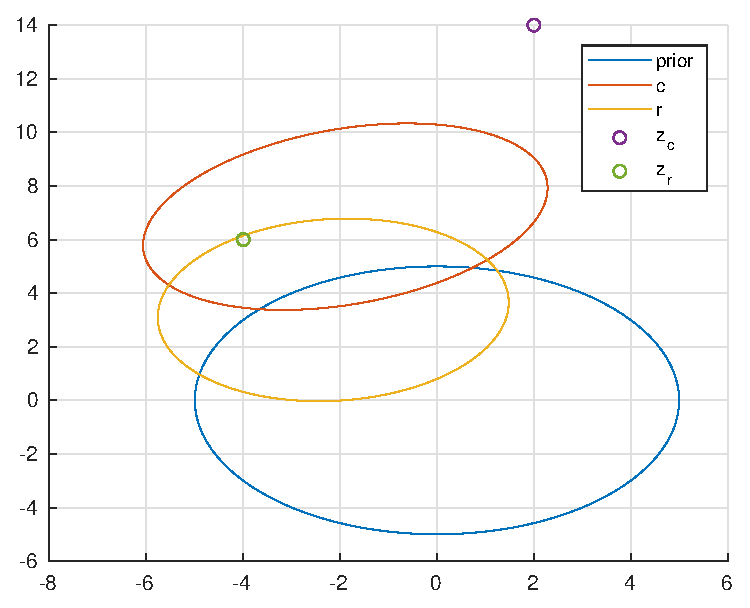
\includegraphics[width=\maxwidth{56.196688409433015em}]{figure_1}
\end{center}


\begin{matlabcode}
% task 5 (g)

% condition the already camera conditioned on the radar
x_bar_cr = condition_mean(x_bar_c, z_r, P_c, H_r, R_r)
\end{matlabcode}
\begin{matlaboutput}
x_bar_cr =
   -2.7183
    6.4872

\end{matlaboutput}
\begin{matlabcode}
P_cr =  condition_cov(P_c, H_r, R_r)
\end{matlabcode}
\begin{matlaboutput}
P_cr =
   10.7043    2.3261
    2.3261    7.7676

\end{matlaboutput}
\begin{matlabcode}

% condition the already radar conditioned on the camera
x_bar_rc = condition_mean(x_bar_r, z_c, P_r, H_c, R_c)
\end{matlabcode}
\begin{matlaboutput}
x_bar_rc =
   -2.7183
    6.4872

\end{matlaboutput}
\begin{matlabcode}
P_rc = condition_cov(P_r, H_c, R_c)
\end{matlabcode}
\begin{matlaboutput}
P_rc =
   10.7043    2.3261
    2.3261    7.7676

\end{matlaboutput}
\begin{matlabcode}

% Plot 1 sigma ellipses
figure(3); clf; hold on; grid on;

data = x_bar + chol(P)' * circle;
plot(data(1,:), data(2, :), 'DisplayName','prior')

data = x_bar_c + chol(P_c)' * circle;
plot(data(1,:), data(2, :), 'DisplayName', 'c')

data = x_bar_r + chol(P_r)' * circle;
plot(data(1,:), data(2, :), 'DisplayName', 'r')

data = x_bar_cr + chol(P_c)' * circle;
plot(data(1,:), data(2, :), 'DisplayName', 'cr')

data = x_bar_rc + chol(P_r)' * circle;
plot(data(1,:), data(2, :), 'DisplayName', 'rc')

% meausrements
scatter(z_c(1), z_c(2), 'DisplayName', 'z_c')
scatter(z_r(1), z_r(2), 'DisplayName', 'z_r')

legend()
\end{matlabcode}
\begin{center}
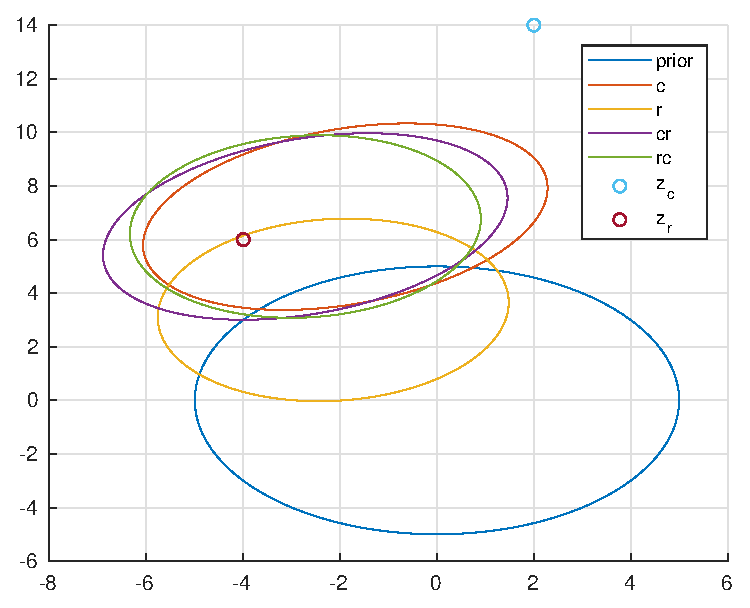
\includegraphics[width=\maxwidth{56.196688409433015em}]{figure_2}
\end{center}

As we can see, it \textit{does} matter in which order we condition, as the distributions are not the same in the resulting plot.

\setcounter{subsection}{7}
\subsection{}
As we can see from figure \ref{fig:bigprob}, big prob.
\begin{figure}[H]
\centering
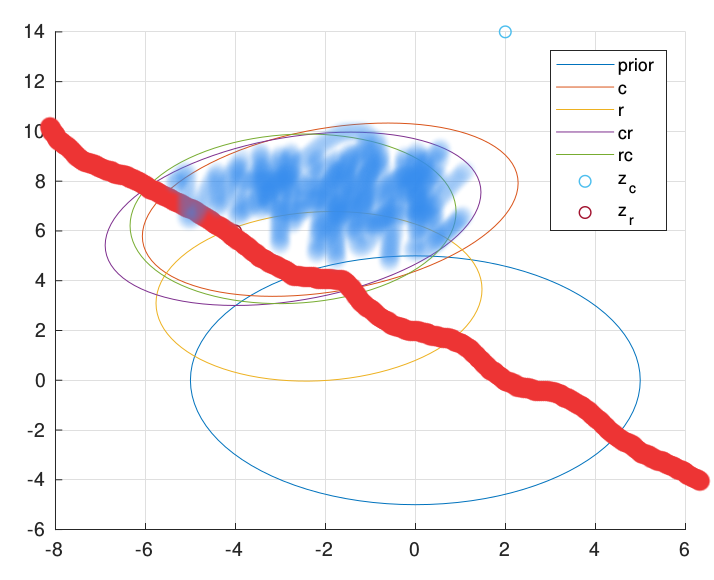
\includegraphics[width=\columnwidth]{bigprob.png}
\caption{Big prob.}
\label{fig:bigprob}
\end{figure}

\end{document}

